\documentclass[10pt,conference,letterpaper]{IEEEtran}

\IEEEoverridecommandlockouts
\usepackage{amsmath,amssymb}
\usepackage{booktabs}
\usepackage{cite}
\usepackage{graphicx}
\usepackage{url}

\title{Smart-CALM: ACK-Aware Online Redundancy Control for Airtime-Constrained LoRa Mesh Networks}

\author{
\IEEEauthorblockN{Author Name}
\IEEEauthorblockA{Department or Laboratory, Institution\\
City, Country\\
Email: your.email@example.com}
}

\begin{document}
\maketitle

\begin{abstract}
Low-power LoRa mesh networks extend coverage beyond a single radio hop, but
each relay consumes long airtime on a shared and collision-prone channel.
Flooding protects delivery at high channel cost, whereas cached source routes
are efficient but can fail when links age or acknowledgments are lost. We
present Smart-CALM, an ACK-aware online redundancy controller that selects
among lean, balanced, and rescue forwarding profiles using a compact
node-local tabular policy. The data plane retains explicit source-route
discovery, bounded fallback forwarding, and reverse-path end-to-end ACKs. The
controller uses recent delivery, route-cache, collision, and delay signals to
adapt route lifetime, discovery timing, and timeout-rescue radius. In a
packet-level LoRa simulation with 50 nodes and 20 common random seeds per
scenario, Smart-CALM improves ACK-confirmed unicast delivery over flooding,
source-route caching, and nonadaptive CALM in repeated-unicast, mixed-traffic,
and stronger-shadowing scenarios. In mixed traffic it reaches 0.937 ACK PDR
with 836.6 s of airtime, compared with 0.852 and 1182.9 s for managed
flooding. The gain is not free: the adaptive method produces a longer tail ACK
delay and spends more fallback forwarding than CALM. We therefore frame the
result as a reliability-airtime-delay tradeoff and release the complete
reproducible comparison matrix.
\end{abstract}

\begin{IEEEkeywords}
LoRa mesh, low-power IoT, adaptive routing, online learning, ACK-aware
reliability, airtime control
\end{IEEEkeywords}

\section{Introduction}

LoRa is attractive for sparse Internet-of-Things deployments because a low
data rate can be exchanged for long range and low endpoint power
\cite{augustin2016study}. A single-hop star, however, is not sufficient when
terrain, buildings, or deployment cost prevent every sensor from reaching a
gateway. Multihop and mesh extensions therefore remain an active design space
\cite{cotrim2020lorawanmesh,centelles2021beyond,wong2024multihop}. Their
central systems problem is that a relay improves reachability by consuming
additional airtime on a channel where packets are long and overlapping
transmissions are expensive.


Two common design points expose this tension. Managed flooding provides
multiple forwarding opportunities and can preserve delivery when a single
route is weak, but duplicate receptions and rebroadcasts increase channel
occupancy. Route discovery followed by source-route caching reduces repeated
control traffic, but a cached path is vulnerable to link variation, aging, and
an ACK that is lost after the destination has already received DATA. Existing
LoRa mesh work explores distance-vector routing, clustering, real-time
forwarding, and implementation tradeoffs
\cite{pueyo2024minimalistic,zhu2019improving,ahmar2022smarthop,leonardi2023mrt,sole2022implementation};
the remaining design question is how much redundancy to spend after the
network has evidence that a path is becoming unreliable.


This paper presents Smart-CALM, a confidence-aware LoRa mesh controller that
treats forwarding redundancy as a resource allocated from delivery evidence.
The method does not require a global topology service or a neural model. A
source first uses source-route forwarding. A compact node-local controller
observes ACK-confirmed outcomes, route-cache behavior, collision pressure, and
delay, then selects one of three prevalidated profiles. A delayed fallback
transmission is scheduled only when the selected profile permits it; an ACK
received before the fallback cancels that redundant transmission. A timeout
rescue uses a profile-specific fallback radius, while first-contact route-miss
recovery remains conservative.


The contributions are:
\begin{enumerate}
\item an ACK-aware redundancy controller that separates destination DATA
arrival from source-confirmed application delivery;
\item a small state/action/reward formulation that is implementable on
MCU-class nodes and changes only a few data-plane parameters;
\item a reproducible seven-configuration comparison covering baselines,
ablations, common-random-number scenarios, and stress conditions; and
\item an explicit analysis of the reliability-airtime-delay tradeoff, including
the cases where Smart-CALM does not dominate every metric.
\end{enumerate}

\section{Problem and Design Goals}

\subsection{Reliability Has Two Observable Endpoints}

For a unicast flow, the destination can receive DATA even when the source
never receives the returning ACK. Reporting only destination arrival would
therefore overstate application-level reliability. Let $F$ be the set of
unicast flows, $D$ the flows whose DATA reaches the destination, and $A$ the
flows whose ACK reaches the source. We report
\begin{equation}
 \mathrm{PDR}_{\mathrm{ACK}} = \frac{|A|}{|F|}, \qquad
 \mathrm{PDR}_{\mathrm{DATA}} = \frac{|D|}{|F|}.
\end{equation}
The first quantity is the primary application-level metric. The second
diagnoses failures in the reverse ACK path and prevents the controller from
confusing destination reachability with confirmed delivery.


\subsection{Resource-Constrained Objective}

The controller seeks high confirmed delivery while limiting airtime,
collisions, route repairs, fallback redundancy, and delay. A useful abstract
objective is
\begin{equation}
 J = \lambda_d \mathrm{PDR}_{\mathrm{ACK}}
 - \lambda_a T_{\mathrm{air}}
 - \lambda_c C
 - \lambda_r R
 - \lambda_f F_{\mathrm{fallback}}
 - \lambda_\ell \bar{L},
\end{equation}
where $T_{\mathrm{air}}$ is total time on air, $C$ is collision pressure, $R$
is route-repair activity, $F_{\mathrm{fallback}}$ is fallback forwarding, and
$\bar{L}$ is observed delivery delay. Smart-CALM does not solve this objective
globally; it uses a small online approximation to choose among bounded
profiles. This keeps the control surface narrow enough for a direct-radio
firmware implementation.


\section{Smart-CALM Design}

\begin{figure*}[t]
\centering
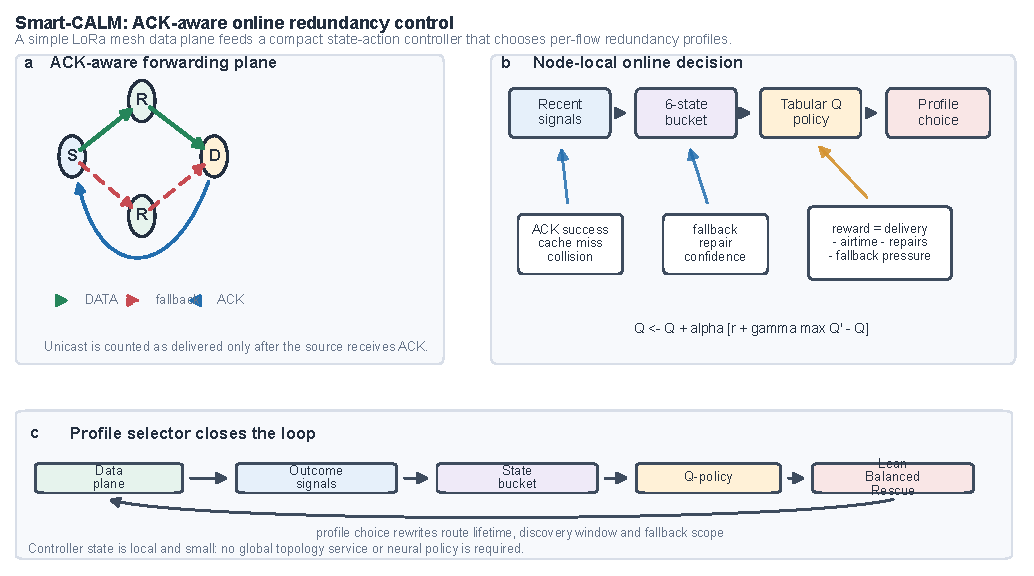
\includegraphics[width=\textwidth]{figures/fig_smart_calm_architecture.pdf}
\caption{Smart-CALM architecture. The forwarding plane exposes source-routed
DATA, bounded fallback, and reverse-path ACKs. A node-local controller buckets
recent outcomes, updates a compact tabular policy, and selects a profile that
changes route lifetime, discovery timing, and timeout-rescue scope.}
\label{fig:architecture}
\end{figure*}

\subsection{Forwarding Plane}

Smart-CALM uses a four-message data plane: route request (RREQ), route reply
(RREP), DATA, and ACK. A source without a valid route floods an RREQ. Candidate
paths reaching the destination are retained during a short discovery window;
the source then selects the candidate with the highest estimated confidence,
breaking ties by hop count. The RREP returns along the reverse path and
installs a source-route cache entry.


Subsequent DATA packets carry the complete path. The destination emits an ACK
on the reverse path, and the source marks the flow delivered only when that ACK
arrives. This is intentionally stricter than counting destination reception.
For a path that is weak or stale, Smart-CALM may schedule a second FALLBACK
transmission after a delay based on the path airtime. FALLBACK is a bounded
managed flood with duplicate suppression. If the source receives the ACK
before the delayed fallback begins, the pending fallback is cancelled. This
coupling prevents a successful source route from needlessly adding a second
flood.


\subsection{Path Confidence}

For a received packet, let $m$ be the SNR margin relative to the demodulation
threshold and let $I_c$ indicate a collision. The link confidence used during
route discovery is
\begin{equation}
 c_{\ell} = \mathrm{clip}\left(
 \frac{1}{1+\exp(-0.7m)} - 0.18 I_c,\;0.05,\;0.98\right).
\end{equation}
For a candidate path $p$, the inherited confidence is the minimum hop
confidence, with a hop penalty:
\begin{equation}
 c(p) = \mathrm{clip}\left(
 \min_{\ell\in p}c_{\ell} - 0.025(|p|-2),\;0.05,\;0.98\right).
\end{equation}
Cached routes are aged by a normalized lifetime penalty. The resulting score
is used for route selection and for deciding whether a bounded fallback should
be scheduled. Confidence is not a guarantee of delivery; it is a local signal
that lets redundancy respond to link evidence.


\subsection{Profiles and Timeout Rescue}

The controller selects one of three profiles:
\begin{itemize}
\item \emph{lean}: 900 s route lifetime, 1-hop timeout rescue, and low path
penalties;
\item \emph{balanced}: 600 s route lifetime, 2-hop timeout rescue, and the
default discovery and aging parameters; and
\item \emph{rescue}: 360 s route lifetime, a 2.8 s discovery window, and
3-hop timeout rescue after a low-confidence observation.
\end{itemize}
The profiles are not separate protocols. They are bounded parameter sets for
the same forwarding plane. The route-miss path remains conservative and uses
the maximum hop budget unless an explicit experiment option overrides it. The
v2 implementation evaluated here applies the selected profile mainly to
per-flow route lifetime, confidence handling, and late timeout rescue. This
distinction matters because reducing first-contact discovery scope would
confound efficiency with reachability.


\subsection{Online Policy}

Every 30 s, the controller aggregates a snapshot of recent metrics. The
reliability bucket is low, medium, or high based on ACK PDR and route-cache
miss ratio. A second bit records whether the collision rate exceeds 0.18,
giving six states. The action is one of the three profiles. The window reward
is
\begin{align}
 r ={}&1.6p_{\mathrm{ACK}} + 0.4g_{\mathrm{broadcast}}
 -0.03\bar{L} -0.35\rho_{\mathrm{control}} \nonumber\\
 &-0.012\rho_{\mathrm{collision}} -0.05N_{\mathrm{repair}}
 -0.004N_{\mathrm{fallback}} .
\end{align}
The tabular update is
\begin{equation}
 Q(s,a) \leftarrow Q(s,a) + \alpha
 [r+\gamma\max_{a'}Q(s',a')-Q(s,a)],
\end{equation}
with $\alpha=0.45$ and $\gamma=0.75$ in the default implementation. A small
exploration probability is retained, and a weak profile bias favors lean
actions when values are tied. The fixed-profile ablation uses the balanced
profile without online switching. The no-fallback ablation disables bounded
rescue, and the no-confidence ablation selects the shortest route candidate
instead of the highest-confidence candidate.


\section{Experimental Method}

\subsection{Packet-Level LoRa Model}

We use the repository's discrete-event packet-level simulator. Nodes are
placed in a 3000 m square. Propagation uses log-distance path loss with
log-normal shadowing. The PHY is fixed at SF9, 125 kHz bandwidth, coding rate
4/5, 17 dBm transmit power, and 32-byte payloads. The channel is half-duplex,
and overlapping packets fail unless the desired signal exceeds the strongest
interferer by a 6 dB capture threshold. Airtime follows the standard LoRa
symbol and payload calculation \cite{semtech2013lora}; the radio parameter
names and current assumptions are aligned with an SX1262-class device
\cite{semtech2024sx1262}.


All protocol runs for a given seed share node placement, traffic schedule,
PHY settings, and a static per-link shadowing realization. This common-random-
number design reduces variance in protocol differences. The simulator is a
research model, not a waveform emulator and not a line-by-line implementation
of Meshtastic or MeshCore. The two named baselines are behavior-equivalent
models: managed flooding and route discovery plus source-route caching.


\subsection{Comparison Matrix}

The matrix contains seven configurations: Meshtastic-like managed flooding,
MeshCore-like route caching, nonadaptive CALM, full Smart-CALM, and three
Smart-CALM ablations. We use four scenarios, each with 20 seeds:
\begin{enumerate}
\item repeated unicast at 6 messages/min;
\item mixed unicast/broadcast traffic at 6 messages/min;
\item mixed traffic with shadowing increased from 4 to 6 dB; and
\item mixed traffic at 10 messages/min.
\end{enumerate}
Each run lasts 1200 s with eight fixed unicast pairs. The resulting raw CSV
contains 140 records per scenario (seven configurations times 20 seeds).


\begin{table}[t]
\caption{Default simulation configuration.}
\label{tab:config}
\centering
\footnotesize
\begin{tabular}{ll}
\toprule
\textbf{Parameter} & \textbf{Value}\\
\midrule
Nodes / area & 50 / $3000\,\mathrm{m}\times3000\,\mathrm{m}$\\
Duration / seeds & 1200 s / 20\\
Unicast pairs / load & 8 / 6 or 10 messages/min\\
PHY & SF9, BW 125 kHz, CR 4/5\\
Payload / transmit power & 32 bytes / 17 dBm\\
Path loss / shadowing & 2.7 / 4 or 6 dB\\
Capture threshold & 6 dB\\
Energy model & 120 mA Tx, 10.3 mA Rx, 3.3 V\\
\bottomrule
\end{tabular}
\end{table}


\subsection{Metrics and Statistics}

For every seed we record the two unicast reliability measures, broadcast
coverage, mean and P95 delivery/ACK delay, transmission counts, total airtime,
channel busy ratio, energy, packet reception ratio, collision rate, route
repairs, fallback forwarding, and policy telemetry. Energy is an accounting
model based on the stated transmit and receive currents; it is not a board
measurement. For each protocol and metric, we report the mean, sample standard
deviation, and a two-sided 95\% Student-$t$ interval over the 20 seeds.


\section{Results}

\subsection{Mixed-Traffic Main Comparison}

Table~\ref{tab:mixed} shows the main mixed-traffic result. Smart-CALM obtains
0.937 ACK PDR, exceeding managed flooding by 0.085 and CALM by 0.202, while
using 29.3\% less airtime than managed flooding. Its total energy is close to
CALM, but its P95 ACK delay is 14.773 s because the metric includes late
rescue and reverse-path confirmation. The result is therefore a reliability
gain with a tail-latency cost.


\begin{table*}[t]
\caption{Mixed-traffic comparison, means over 20 seeds.}
\label{tab:mixed}
\centering
\scriptsize
\resizebox{\textwidth}{!}{%
\begin{tabular}{lrrrrrrr}
\toprule
\textbf{Protocol} & \textbf{ACK PDR} & \textbf{DATA PDR} &
\textbf{P95 ACK delay (s)} & \textbf{Airtime (s)} &
\textbf{Collision rate} & \textbf{Fallback fwd.} & \textbf{Energy (J)}\\
\midrule
Meshtastic-like & 0.852 & 0.955 & 1.119 & 1182.9 & 0.526 & 0.0 & 2017.2\\
MeshCore-like & 0.389 & 0.661 & 0.646 & 971.5 & 0.427 & 0.0 & 1578.8\\
CALM & 0.735 & 0.769 & 2.740 & 839.6 & 0.443 & 50.5 & 1384.5\\
Smart-CALM & \textbf{0.937} & \textbf{0.967} & 14.773 & \textbf{836.6} &
0.449 & 104.2 & 1388.5\\
Smart-CALM static & 0.941 & 0.957 & 15.794 & 913.6 & 0.449 & 357.1 & 1512.5\\
Smart-CALM no-fallback & 0.768 & 0.797 & 2.608 & 828.6 & 0.450 & 64.8 & 1371.5\\
Smart-CALM no-confidence & 0.937 & 0.967 & 14.773 & 836.6 & 0.449 & 104.2 & 1388.5\\
\bottomrule
\end{tabular}}
\end{table*}


\subsection{Scenario Robustness}

Table~\ref{tab:scenarios} compresses the four scenario means for the primary
reliability and airtime metrics. Smart-CALM remains above CALM and
MeshCore-like on ACK PDR in every scenario. Under stronger shadowing its ACK
PDR is 0.928, while managed flooding reaches 0.842. Under the 10 messages/min
load, all methods degrade, but Smart-CALM retains 0.871 ACK PDR versus 0.571
for CALM and 0.364 for MeshCore-like. The higher-load result also raises
Smart-CALM airtime to 1344.9 s, showing that rescue forwarding spends more
channel resources as reliability becomes harder to maintain.


\begin{table*}[t]
\caption{Primary metrics across all scenarios, means over 20 seeds.}
\label{tab:scenarios}
\centering
\scriptsize
\resizebox{\textwidth}{!}{%
\begin{tabular}{llrrrrrr}
\toprule
\textbf{Scenario} & \textbf{Protocol} & \textbf{ACK PDR} &
\textbf{DATA PDR} & \textbf{P95 ACK delay (s)} & \textbf{Airtime (s)} &
\textbf{Collision rate} & \textbf{Energy (J)}\\
\midrule
Repeated unicast & Meshtastic-like & 0.838 & 0.949 & 1.769 & 1152.0 & 0.526 & 1976.6\\
Repeated unicast & MeshCore-like & 0.605 & 0.812 & 0.592 & 357.8 & 0.388 & 603.0\\
Repeated unicast & CALM & 0.831 & 0.856 & 2.740 & 256.3 & 0.345 & 438.0\\
Repeated unicast & Smart-CALM & \textbf{0.936} & \textbf{0.961} & 14.876 & 289.6 & 0.351 & 498.5\\
\midrule
Mixed traffic & Meshtastic-like & 0.852 & 0.955 & 1.119 & 1182.9 & 0.526 & 2017.2\\
Mixed traffic & MeshCore-like & 0.389 & 0.661 & 0.646 & 971.5 & 0.427 & 1578.8\\
Mixed traffic & CALM & 0.735 & 0.769 & 2.740 & 839.6 & 0.443 & 1384.5\\
Mixed traffic & Smart-CALM & \textbf{0.937} & \textbf{0.967} & 14.773 & \textbf{836.6} & 0.449 & 1388.5\\
\midrule
Shadowing 6 dB & Meshtastic-like & 0.842 & 0.949 & 1.236 & 1175.1 & 0.529 & 2008.1\\
Shadowing 6 dB & MeshCore-like & 0.387 & 0.662 & 0.622 & 969.6 & 0.428 & 1575.7\\
Shadowing 6 dB & CALM & 0.731 & 0.775 & 2.740 & 833.8 & 0.447 & 1378.3\\
Shadowing 6 dB & Smart-CALM & \textbf{0.928} & \textbf{0.960} & 14.673 & 842.6 & 0.445 & 1395.8\\
\midrule
Mixed, 10/min & Meshtastic-like & 0.714 & 0.914 & 2.037 & 1876.9 & 0.546 & 3234.0\\
Mixed, 10/min & MeshCore-like & 0.364 & 0.530 & 0.945 & 1442.7 & 0.448 & 2368.5\\
Mixed, 10/min & CALM & 0.571 & 0.633 & 2.740 & 1266.8 & 0.470 & 2112.6\\
Mixed, 10/min & Smart-CALM & \textbf{0.871} & \textbf{0.920} & 18.199 & 1344.9 & 0.469 & 2254.2\\
\bottomrule
\end{tabular}}
\end{table*}


\subsection{Ablation Findings}

The ablations help separate the source of the reliability gain. In mixed
traffic, disabling fallback reduces ACK PDR from 0.937 to 0.768 while
reducing airtime only slightly, which indicates that bounded rescue is doing
real recovery work. The static balanced profile reaches a similar PDR but uses
913.6 s of airtime and 357.1 fallback forwards, compared with 836.6 s and
104.2 for the adaptive controller. This supports the claim that profile
selection controls redundancy rather than merely enabling a permanently
aggressive mode.


The confidence-ranking ablation is currently identical to Smart-CALM in the
first three scenarios and differs only slightly at high load. This is not
evidence that confidence ranking is useless. It means the sampled topologies
rarely contain a strong conflict between path length and confidence. A targeted
topology with two competing routes is required before making a stronger
ablation claim.


\section{Discussion and Limitations}

\subsection{Interpreting the Tradeoff}

Smart-CALM's primary advantage is not a universal reduction in every cost.
Compared with managed flooding, it cuts mixed-traffic airtime by 346.4 s while
raising ACK PDR by 0.085. Compared with CALM, it raises ACK PDR by 0.202 at
almost the same airtime, but its P95 ACK delay is more than five times larger.
The mechanism spends this delay on delayed fallback and ACK confirmation.
Applications with a strict latency deadline may prefer CALM or the no-fallback
variant; applications that value confirmed delivery under unstable paths may
prefer Smart-CALM.


\subsection{Reproducibility and Scope}

The complete matrix is generated by a shell script and stored as raw
per-seed CSV plus long-format summary CSV. The simulator uses fixed random
seeds and common propagation realizations across protocols. These controls make
the comparison auditable, but they do not turn a packet-level model into a
physical LoRa testbed. The energy values use 120 mA transmit current, 10.3 mA
receive current, and 3.3 V; board startup, sleep current, antenna mismatch,
and channel-regulatory duty-cycle effects are outside the model.


The evaluated scale is 50 nodes in a square area. The results do not establish
scalability to hundreds of nodes, dense interference environments, or changing
traffic beyond the tested load. The baselines are behavior-equivalent models,
not claims of compatibility with the Meshtastic or MeshCore wire protocols.
Finally, the confidence-ranking ablation needs a deliberately constructed
route-conflict scenario, and the firmware prototype still requires
board-level radio validation before deployment claims are warranted.


\section{Related Work}

LoRa and LoRaWAN surveys describe the sensitivity of long-range low-rate
systems to airtime, gateway reachability, and multihop design
\cite{augustin2016study,cotrim2020lorawanmesh,osorio2020routing}. Mesh
extensions have explored distance-vector routing, clustering, and compact
implementation strategies \cite{pueyo2024minimalistic,zhu2019improving,
sole2022implementation}. Smart-Hop and MRT-LoRa address latency and
real-time forwarding concerns \cite{ahmar2022smarthop,leonardi2023mrt}.
Smart-CALM differs in its control boundary: it keeps the forwarding plane
explicit and uses ACK-confirmed outcomes to choose a bounded redundancy
profile at runtime. Its path confidence is also deliberately local and
lightweight, related in spirit to link-quality path metrics such as ETX
\cite{decouto2003etx}, but with an explicit penalty for route age and a
separate ACK endpoint.


\section{Conclusion}

This paper introduced Smart-CALM, an ACK-aware online redundancy controller for
airtime-constrained LoRa mesh networks. Across four 20-seed scenarios, the
method improved source-confirmed delivery over managed flooding, route-cache
forwarding, and nonadaptive CALM while staying below flooding airtime in the
main mixed workload. The results also exposed a meaningful cost: longer tail
ACK delay and more fallback activity. Treating this as a three-way
reliability-airtime-delay tradeoff gives a more defensible contribution than
claiming metric dominance. The next evaluation step is a targeted route
conflict scenario for the confidence ablation, followed by waveform- or
hardware-level validation of the packet-level findings.


\section*{Acknowledgment}

This work uses the MeshEcho open research repository and its reproducible
packet-level simulation harness. Author, affiliation, funding, and conflict
statements remain to be completed before submission.


\bibliographystyle{IEEEtran}
\bibliography{references}


\end{document}
